\documentclass[conference]{IEEEtran}
\IEEEoverridecommandlockouts
\usepackage{cite}
\usepackage{amsmath,amssymb,amsfonts}
\usepackage{algorithmic}
\usepackage{graphicx}
\usepackage{textcomp}
\usepackage{xcolor}
\usepackage{multirow}
\def\BibTeX{{\rm B\kern-.05em{\sc i\kern-.025em b}\kern-.08em
    T\kern-.1667em\lower.7ex\hbox{E}\kern-.125emX}}
\begin{document}

\title{Smart Spreading Factor Assignment for LoRaWANs}


\author{\IEEEauthorblockN{Tugrul Yatagan and Sema F. Oktug}
\IEEEauthorblockA{Department of Computer Engineering,
Istanbul Technical University\\
Istanbul, Turkey\\
Email: \{yatagan, oktug\}@itu.edu.tr}}
\maketitle


\begin{abstract}
Low power wide area network (LPWAN) technologies offer affordable connectivity to massive number of low-power devices distributed over large geographical areas. Focus of this work is one of the most promising LPWAN technologies: LoRa. LoRa offers long range communication and strong resilience to interference by proprietary modulation technique based on Chirp Spread Spectrum (CSS). LoRa modulation trades data rate for sensitivity and communication range by spreading symbols within a fixed channel bandwidth. Collisions in LoRaWAN networks are strongly related with spreading factor (SF) assignment of nodes which indeed effects network performance. In this work, a simulation environment to evaluate the performance of SF assignment schemes is implemented. Furthermore, a novel smart SF assignment strategy which utilizes Support Vector Machine (SVM) and Decision Tree Classifier (DTC) machine learning techniques for optimization of SF assignment is proposed. It is observed and presented that the proposed smart SF assignment techniques give promising simulation results. 
\end{abstract}


\begin{IEEEkeywords}
LoRa, LoRaWAN, Spreading Factor, LPWAN, Machine Learning
\end{IEEEkeywords}


\section{Introduction}
\par In the last few years, number of Internet of Things (IoT) applications increased exponentially \cite{7721743}. Recent developments on LPWAN technologies has great impact on growth of number of IoT applications. LPWAN technologies address some of the well-known wireless communication challenges. Traditional wireless communication methods such as cellular networks (e.g., 2G, 3G, LTE) and short-range communication technologies (e.g., Bluetooth, WiFi, Zigbee) cannot provide low power and long range at the same time. Cellular networks can provide long range and high data rate, but they are complex and consume too much power. Besides, most of the IoT applications do not require high data rate. Short-range communication methods can provide relatively low power consumption, but their range is limited to a few hundred meters at best \cite{7815384}. LPWAN technologies fill the technology gap between short range and cellular technologies by providing low power and long-range communication. LPWAN technologies basically sacrifice data rate to provide low power consumption.

\par There are several emerging LPWAN technologies. LoRa, Sigfox, NB-IoT and LTE-M are commonly used, well-known LPWAN technologies \cite{7815384}. LoRa and Sigfox use license free ISM frequency bands while NB-IoT and LTE-M use licensed frequency bands which brings extra cost \cite{7815384}. Both LoRa and Sigfox are known for ultra-low power consumption and resilience to interference. While NB-IoT and LTE-M are promoted for higher data rate. LoRa has open standard MAC protocol called LoRaWAN. LoRaWAN and Sigfox MAC protocols are based on pure ALOHA medium access. LoRaWAN networks can be deployed as a private network like WiFi. However, Sigfox and NB-IoT are only available with operator contract \cite{7815384}.

\par LoRa can adjust data rate by spreading symbols within a fixed channel bandwidth. This enables tradeoff between receive sensitivity and air time of transmission \cite{7803607}. Simultaneous same SF transmissions are prone to collision, however, different SF transmissions in the same channel are orthogonal to each other. Thus, SF assignment is crucial for overall network performance. In this work, a LoRa discrete event simulator is developed to study the performance of LoRa SF assignment strategies. Also, a machine learning based SF assignment approach is proposed. Support Vector Machine (SVM) and Decision Tree Classifier (DTC) techniques are employed and the introduced schemes are called as smart SF schemes. The performance of the smart schemes is compared with the performance of the lowest SF assignment scheme. It is shown that the proposed smart SF assignment schemes give promising results.

\par This paper is organized as follows: Section \ref{LoRa} and Section \ref{LoRaWAN} provides some background information about LoRa and LoRaWAN. Section \ref{Related Works} summarize  the other related works. Section \ref{Proposed Technique} describes the smart SF assignment technique proposed. Simulation environments and results are shown in Section \ref{Simulation Environment} and \ref{Simulation Results}. Finally, Section \ref{Conclusion} concludes the paper by giving future directions.


\section{LoRa} \label{LoRa}
\par LoRa is a proprietary physical layer radio/chipset technology that provides wireless link solution for LPWANs. It uses proprietary spread spectrum modulation technique that is the derivative of Chirp Spread Spectrum (CSS). A chirp is a sinusoidal signal of which frequency increases over time. Chirp frequency increases linearly and sweeps the entire bandwidth \cite{AN1200.22}.

\subsection{Spreading Factor}
\par The ratio between symbol and chirp rate is equal to $2$\textsuperscript{SF}. SF can take values between 7 to 12. SF also determines data rate of a LoRa transmission \cite{AN1200.22}. Data rate of a LoRa transmission can be calculated as:

\begin{equation} \label{eq:bit_rate_sf}
R_{b} = SF * \dfrac{\left[ \dfrac{4}{4+CR} \right] }{ \left[ \dfrac{2^{SF}}{BW|_{Hz}} \right]} \ bps
\end{equation}

Where, $R_{b}$ is data rate in bps, SF is spreading factor $SF \in \{7,..,12\}$, CR is error correction code rate $CR \in \{1,..,4\}$ and $BW$ is bandwidth in Hertz \cite{AN1200.22}.

\par When BW and CR are constant, as the SF increases, the data rate decreases. Increasing the SF makes the signal more resilient to noise thus increases the transmission range. Increasing the SF also increases the transmission duration which increases the power consumption. Therefore, it is possible to trade between range and power consumption by changing SF.

\subsection{Spreading Factor Assignment Issue}
\par Simultaneous different SF transmissions are orthogonal to each other up to some extent. Which means that, a LoRa GW can simultaneously receive multiple transmissions with different SFs. However, simultaneous transmissions with the same SF may not be received by the GW due to collision. For this reason, SF assignment of nodes is crucial for network performance.

\par In a LoRaWAN network, initially, a node is not aware of how far away it is from a GW. However, a node can guess the distance from a GW by observing received signal power of a downlink transmission. If received signal power of a downlink transmission is too high, then node can decrease its next transmission SF to decrease power consumption. This SF assignment method is called lowest possible SF assignment scheme for the rest of the paper. Lowest possible SF assignment scheme is commonly used in LoRaWAN deployments. GW can request from a node to decrease its SF or transmit power.

\par In Figure \ref{fig:collision}, a LoRaWAN network deployed with a single GW is illustrated. Different color rings represent achievable range of different SFs from the GW and different color circles represent selected SF of the nodes. The end devices close to the GW will fall into lowest SF (SF7) area section. The end devices close to the GW will probably select the lowest SF mot the time. Hence the number of collisions will increase as the number of end devices close to the GW increases.

\begin{figure}
\centering
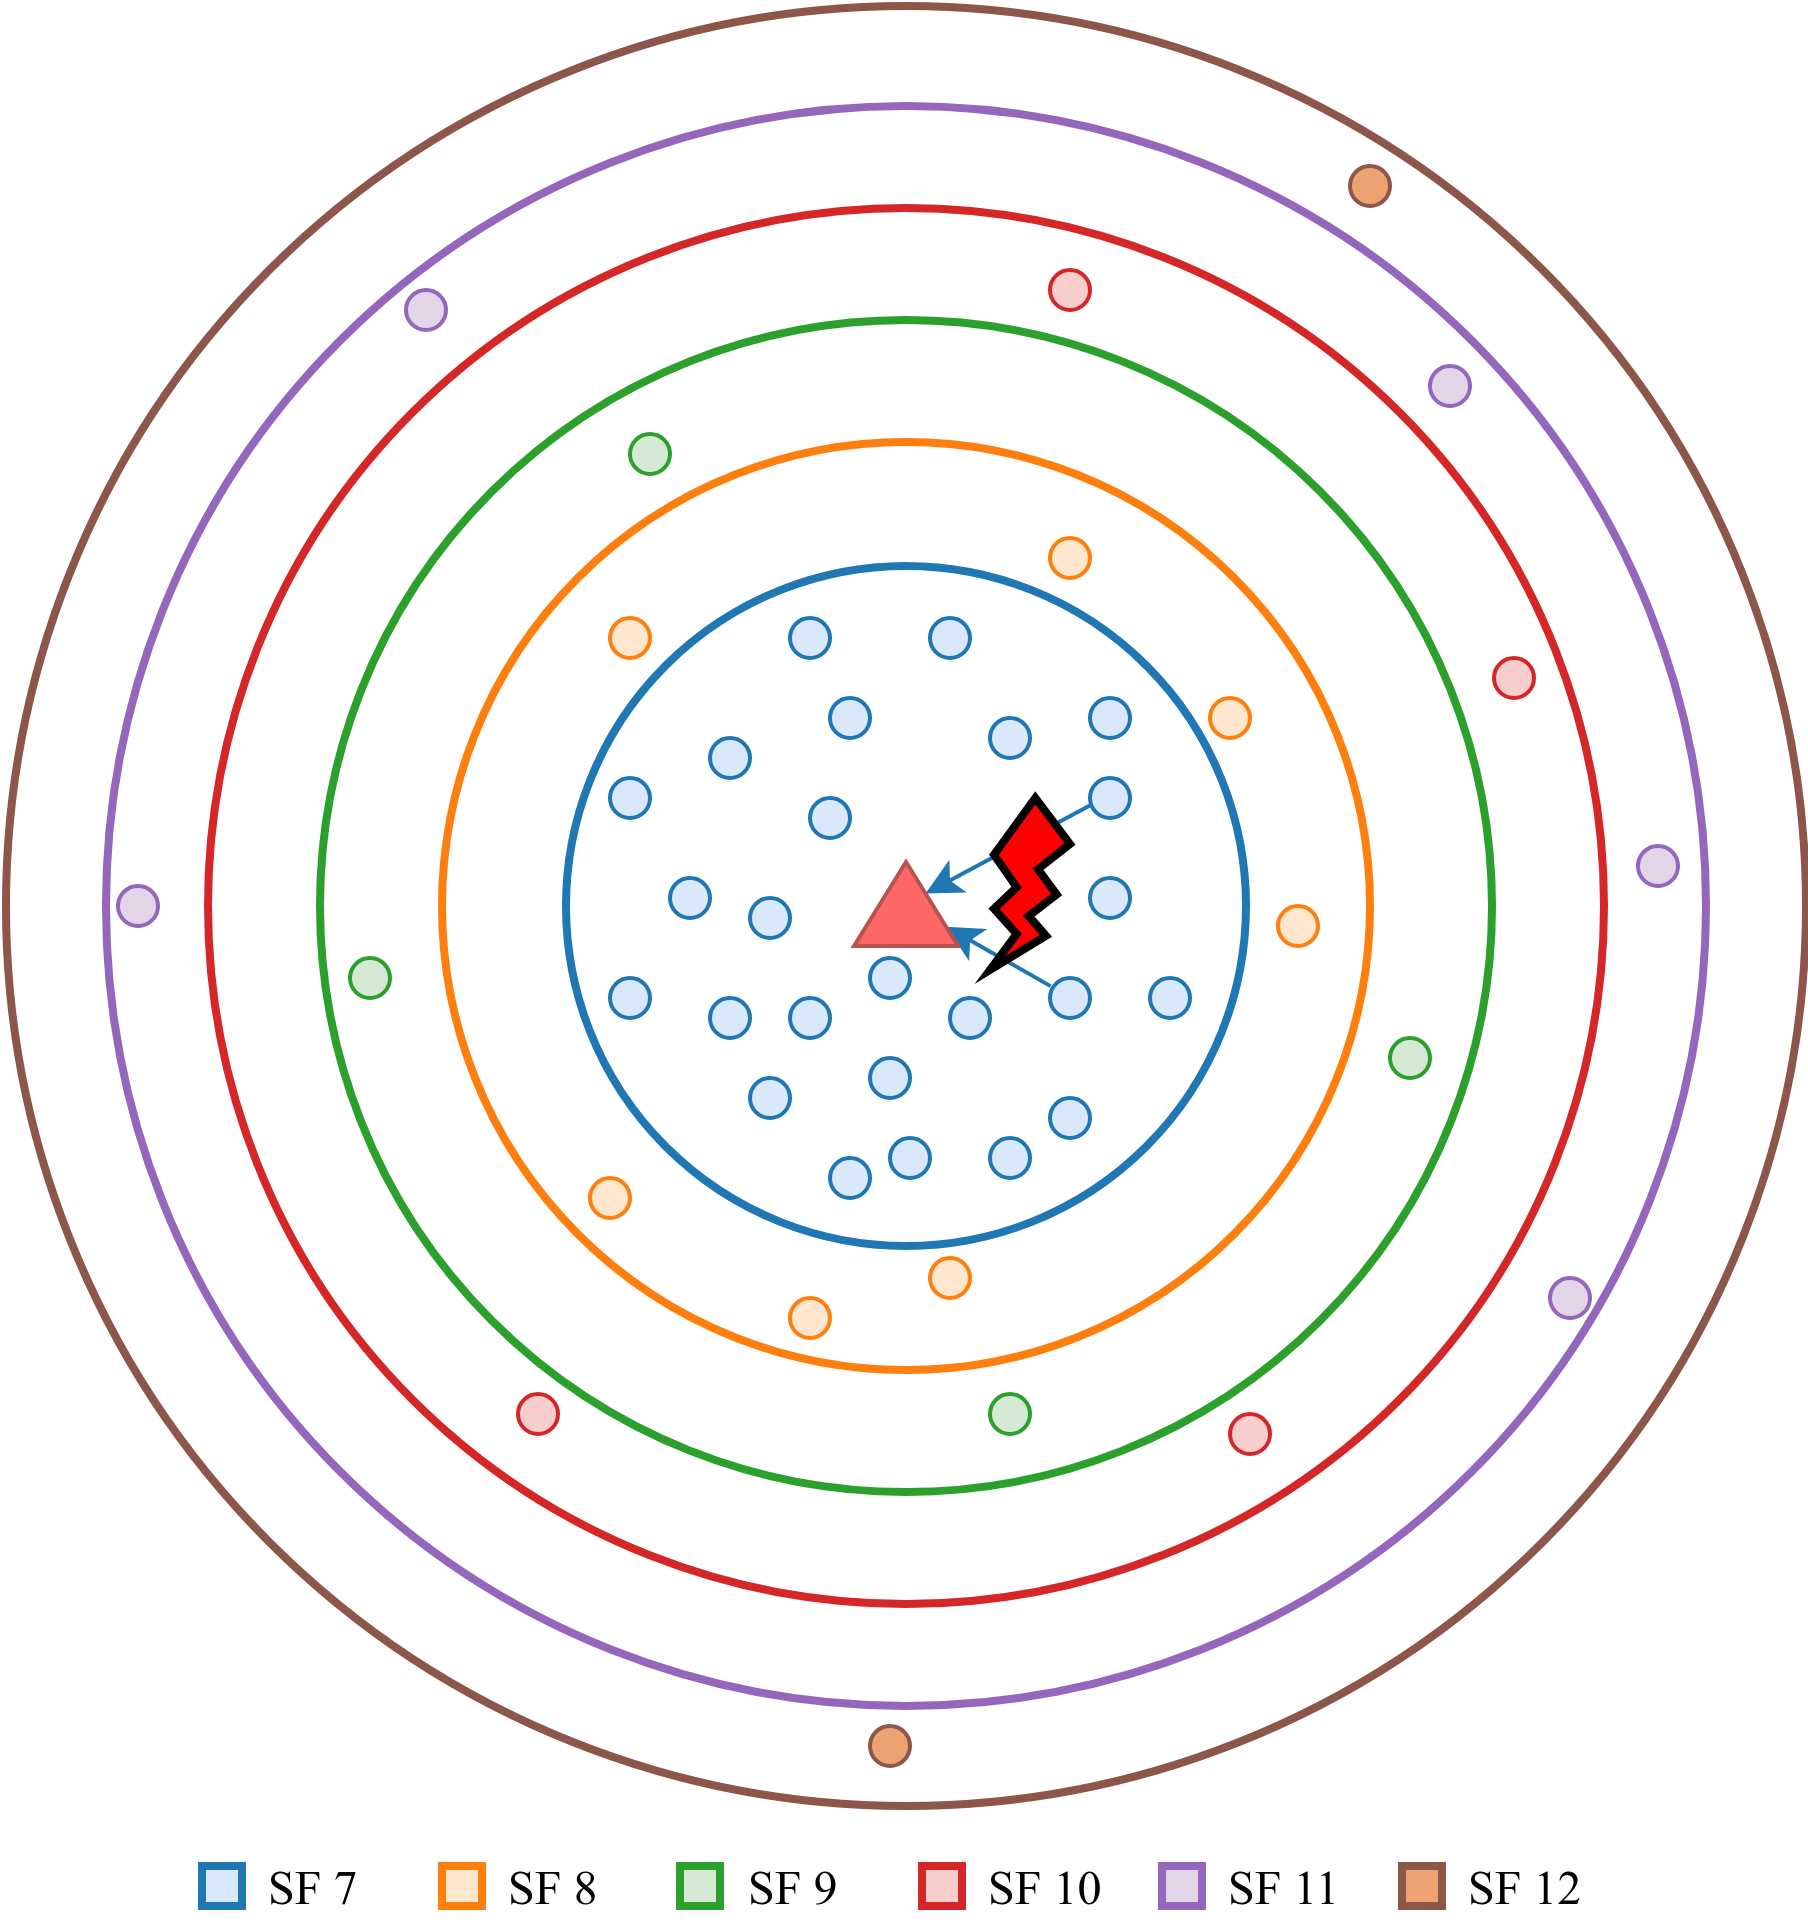
\includegraphics[width=\linewidth]{collision}
\caption{Collision between nodes close to the GW.}
\label{fig:collision}
\end{figure}


\section{LoRaWAN} \label{LoRaWAN}
\par LoRa has an open standard medium access control (MAC) layer protocol called LoRaWAN is which is designed for large scale LoRa networks considering well known LPWAN challenges and their best practice solutions. LoRaWAN is developed and maintained by LoRa Alliance. LoRa Alliance is an open, non-profit organization dedicated to standardization of LoRaWAN. LoRaWAN is based on pure ALOHA medium access which means that end nodes do not check whether the channel is free or not before transmission, accepting the possibility of a collision. A typical LoRaWAN network consists of following three network entities.

\subsection{End node}
\par LoRaWAN end node (EN) is a low power embedded device that only communicates to GWs. LoRaWAN standard defines three classes for end devices which are Class A, Class B, and Class C. Different classes provide LPWAN solutions to different applications and deployments. Class A end nodes generate uplink transmission at any time and only receive a period of time after uplink transmission. Class B end nodes extend Class A behavior by adding scheduled receive windows for downlink transmission. Receive window is synchronized using a beacon packet transmitted by GWs. Class C end nodes extend Class A behavior by keeping receive window open all the time except uplink transmission. This provides Class C end nodes with low latency downlink communication, which it requires more power consumption. In this paper, only Class A end devices are considered since Class A behavior leads to the lowest power consumption.

\subsection{Gateway}
\par LoRaWAN gateway (GW) is a device that communicates with the end nodes. A typical GW can receive from multiple channels at the same time. GWs are usually connected to power grid, so power consumption of a GW is insignificant in most of the deployments.

\subsection{Network server}
\par LoRaWAN network server (NS) is a server that provides MAC layer processing. Network server routes messages from application to end nodes and vice versa. Network server can be used for tweaking end node parameters like channel, transmit power and SF to increase network performance.


\section{Related Works} \label{Related Works}
\par The literature related to the work presented in this paper has started to grow recently. LPWAN technologies and especially LoRa attracted researchers’ attentions lately. Some of these works which studies LoRa/LoRaWAN SF are summarized.

\par In \cite{7996384}, the authors evaluated the performance of LoRaWAN networks in a smart city scenario. The authors proposed a link measurement and a link performance model for LoRa. The authors also proposed a SINR threshold matrix for modeling LoRa interference between simultaneous but different SF LoRa transmissions. They implemented a LoRa simulator in ns-3 to study scalability and performance of LoRaWAN networks. Their results show that SF assignment has great effect on LoRaWAN network performance.

\par In \cite{8090518}, another LoRaWAN ns-3 simulator is presented. Authors introduced an error model for determining range as well as interference between multiple simultaneous LoRa transmissions. Their simulator supports LoRaWAN Class A end devices, multiple GWs, both upstream and downstream confirmed messages. Their results show that allocating network parameters such as SF is highly important for the performance of LoRaWAN networks.

\par In \cite{8267219}, the authors studied the effects of imperfect orthogonality between different LoRa SF transmissions. The authors state that a LoRa transmission can be interfered by a different SF transmission when power of the interfering signal significantly is greater than the reference signal. Their experimental results show that this power difference is around 16 dB such a power difference can be seen when an interfering signal is close to a receiver or the sum of interfering signals' energy can create this power difference.

\par In \cite{8430542}, the authors investigated the impact of the interference caused by simultaneous LoRa transmissions with the same and different SFs. They derived aggregated co-SF and inter-SF interference power SIR distributions to capture the coverage distance from the GW for modeling interference in multiple GWs scenarios. Their results show that transmission among different SFs can cause a significant impact in high-density LoRaWAN networks.


\section{Proposed Technique} \label{Proposed Technique}
\par The collision issue illustrated in Figure \ref{fig:collision} is solved by forcing some of the close nodes to select higher SFs even they are able to communicate with lower SFs. This has potential to prevent collisions due to the orthogonality of the SFs as shown in Figure \ref{fig:collision_solution_single_gw}. Higher SF assigned nodes are drawn with bold circle border in Figure \ref{fig:collision_solution_single_gw}. However, distribution of SF among nodes becomes an important problem. Increasing a node's SF should be done carefully since higher SF means longer air time and longer air time means increasing the probability of collisions with other high SF transmissions. In multiple GWs scenarios, this approach may increase the collisions with the nodes in other GW's range. Thus, extra care should be taken for nodes in the intersection area of the GWs illustrated in Figure \ref{fig:collision_solution_multi_gw}.

\par It is difficult to propose a single SF assignment rule for every possible LoRaWAN topology since every network is different and optimizing their nodes' SFs requires different rules. For this reason, machine learning based SF assignment approach is proposed to decrease the collisions for the same SF transmissions. This technique starts by learning the transmission behavior of the nodes in a network. An NS can keep track of successful uplink transmissions and their SFs. This NS can also keep track of some of the collided transmissions if header part of the packet is not interfered at the GW. However, NS cannot keep track of transmissions with lower receive power than sensitivity of the GW. Using this information, NS can train a classifier to predict future transmission result for a specific node and a specific SF. Using this prediction model NS can assign SFs to nodes considering the collision probability.

\par In this work, decision tree classifier (DTC) and support vector machine (SVM) \cite{Alpaydin} schemes are employed to predict the transmission results. Class weights are balanced according to sample distributions for both methods. For DTC, Gini impurity criteria is used to measure the quality of splits. For SVM, penalty parameter is set to 1, degree is set to 3 and RBF kernel is used.

\par It is possible to generate mass amount of LoRaWAN transmission records for different topologies using our simulator. Data set size is directly proportional to simulation duration. Thus, increasing the simulation duration, improves the prediction accuracy. In real world deployments, NS can keep track of all transmissions and it can create a classifier daily basis, then GWs can request from nodes to use suggested SFs.

\par To come up with a solution for SF assignment, DTC and SVM prediction schemes are integrated to the simulator. A classifier is trained from transmission logs and this classifier is used for selecting optimum SF for the nodes. Simulator first runs a simulation by assigning random SFs to the nodes. Simulation logs are combined into four data columns which are; X and Y coordinates of the transmission source, SF of the transmission and the result of the transmission. Possible transmission results are successful, interfered or under sensitivity. These data are fed to Python scikit-learn DTC or SVM classifiers. After the classifier model is generated, a second simulation is run with classifier. Simulator selects optimum SF considering the prediction of transmission. If a transmission of a node with the lowest possible SF is predicted as interfered by the classifier, then simulator assigns higher SF and evaluates the new prediction. If no SF is predicted as successful, then simulator again assigns the lowest possible SF.

\begin{figure}
\centering
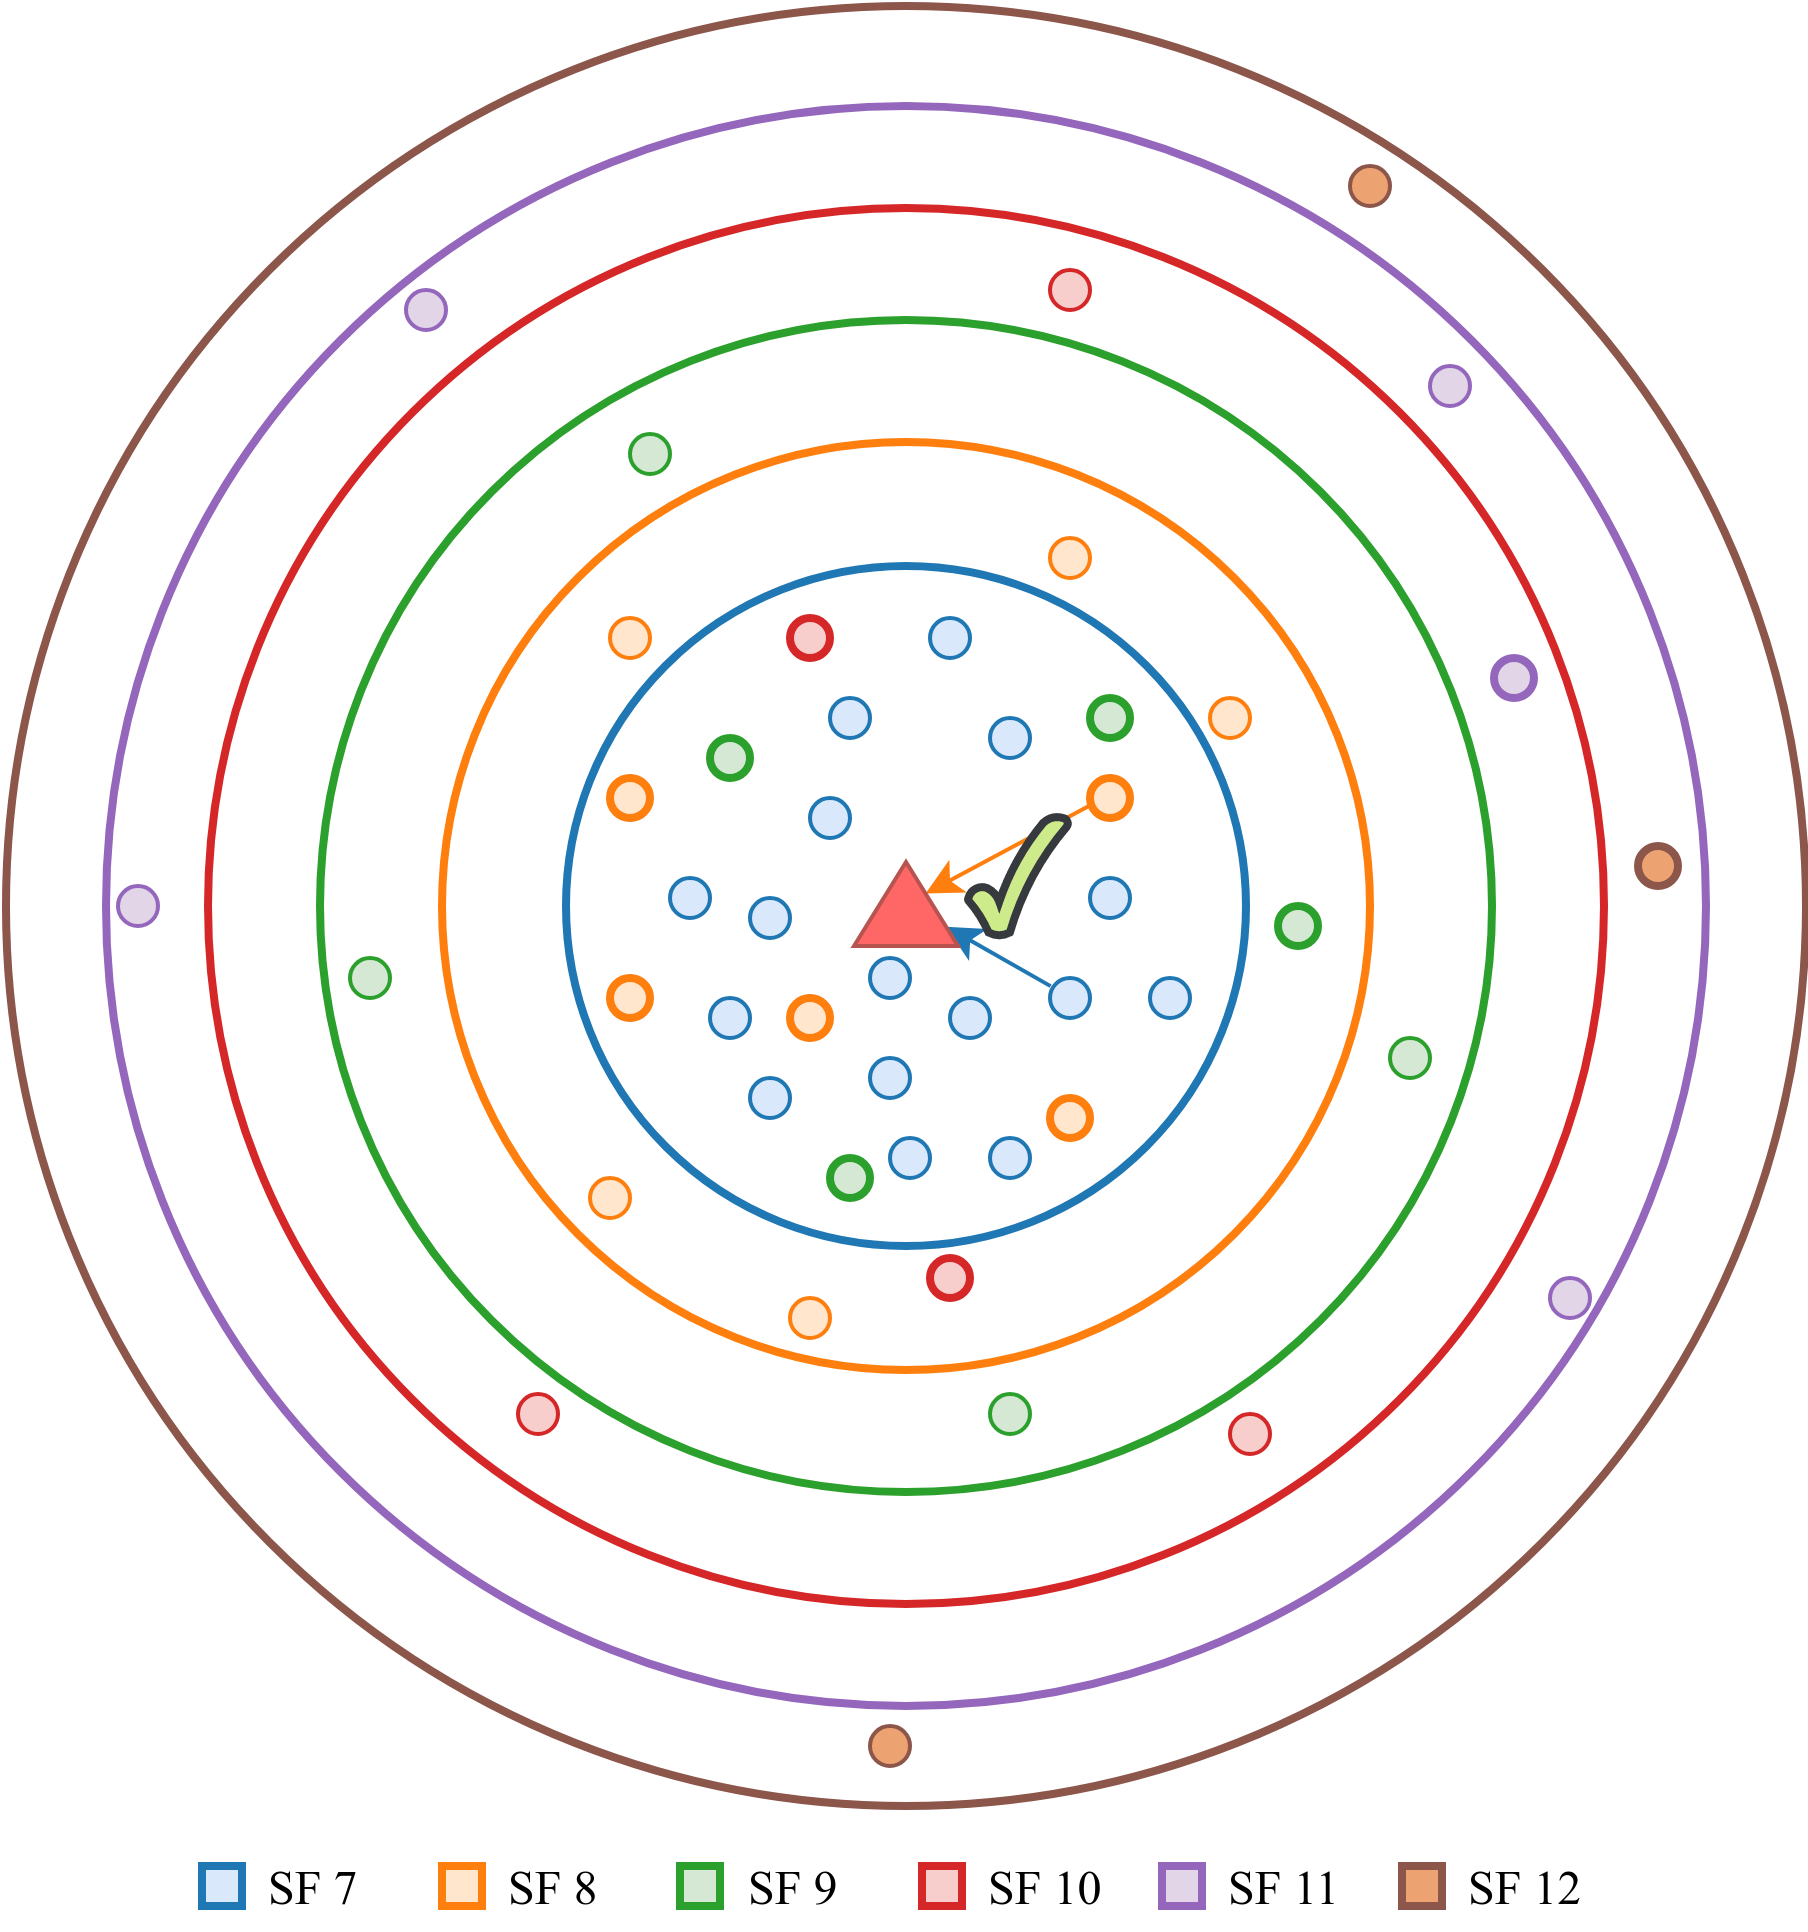
\includegraphics[width=\linewidth]{collision_solution_single_gw}
\caption{Collision avoidance by using higher SF for nodes close to the GW.}
\label{fig:collision_solution_single_gw}
\end{figure}

\begin{figure}
\centering
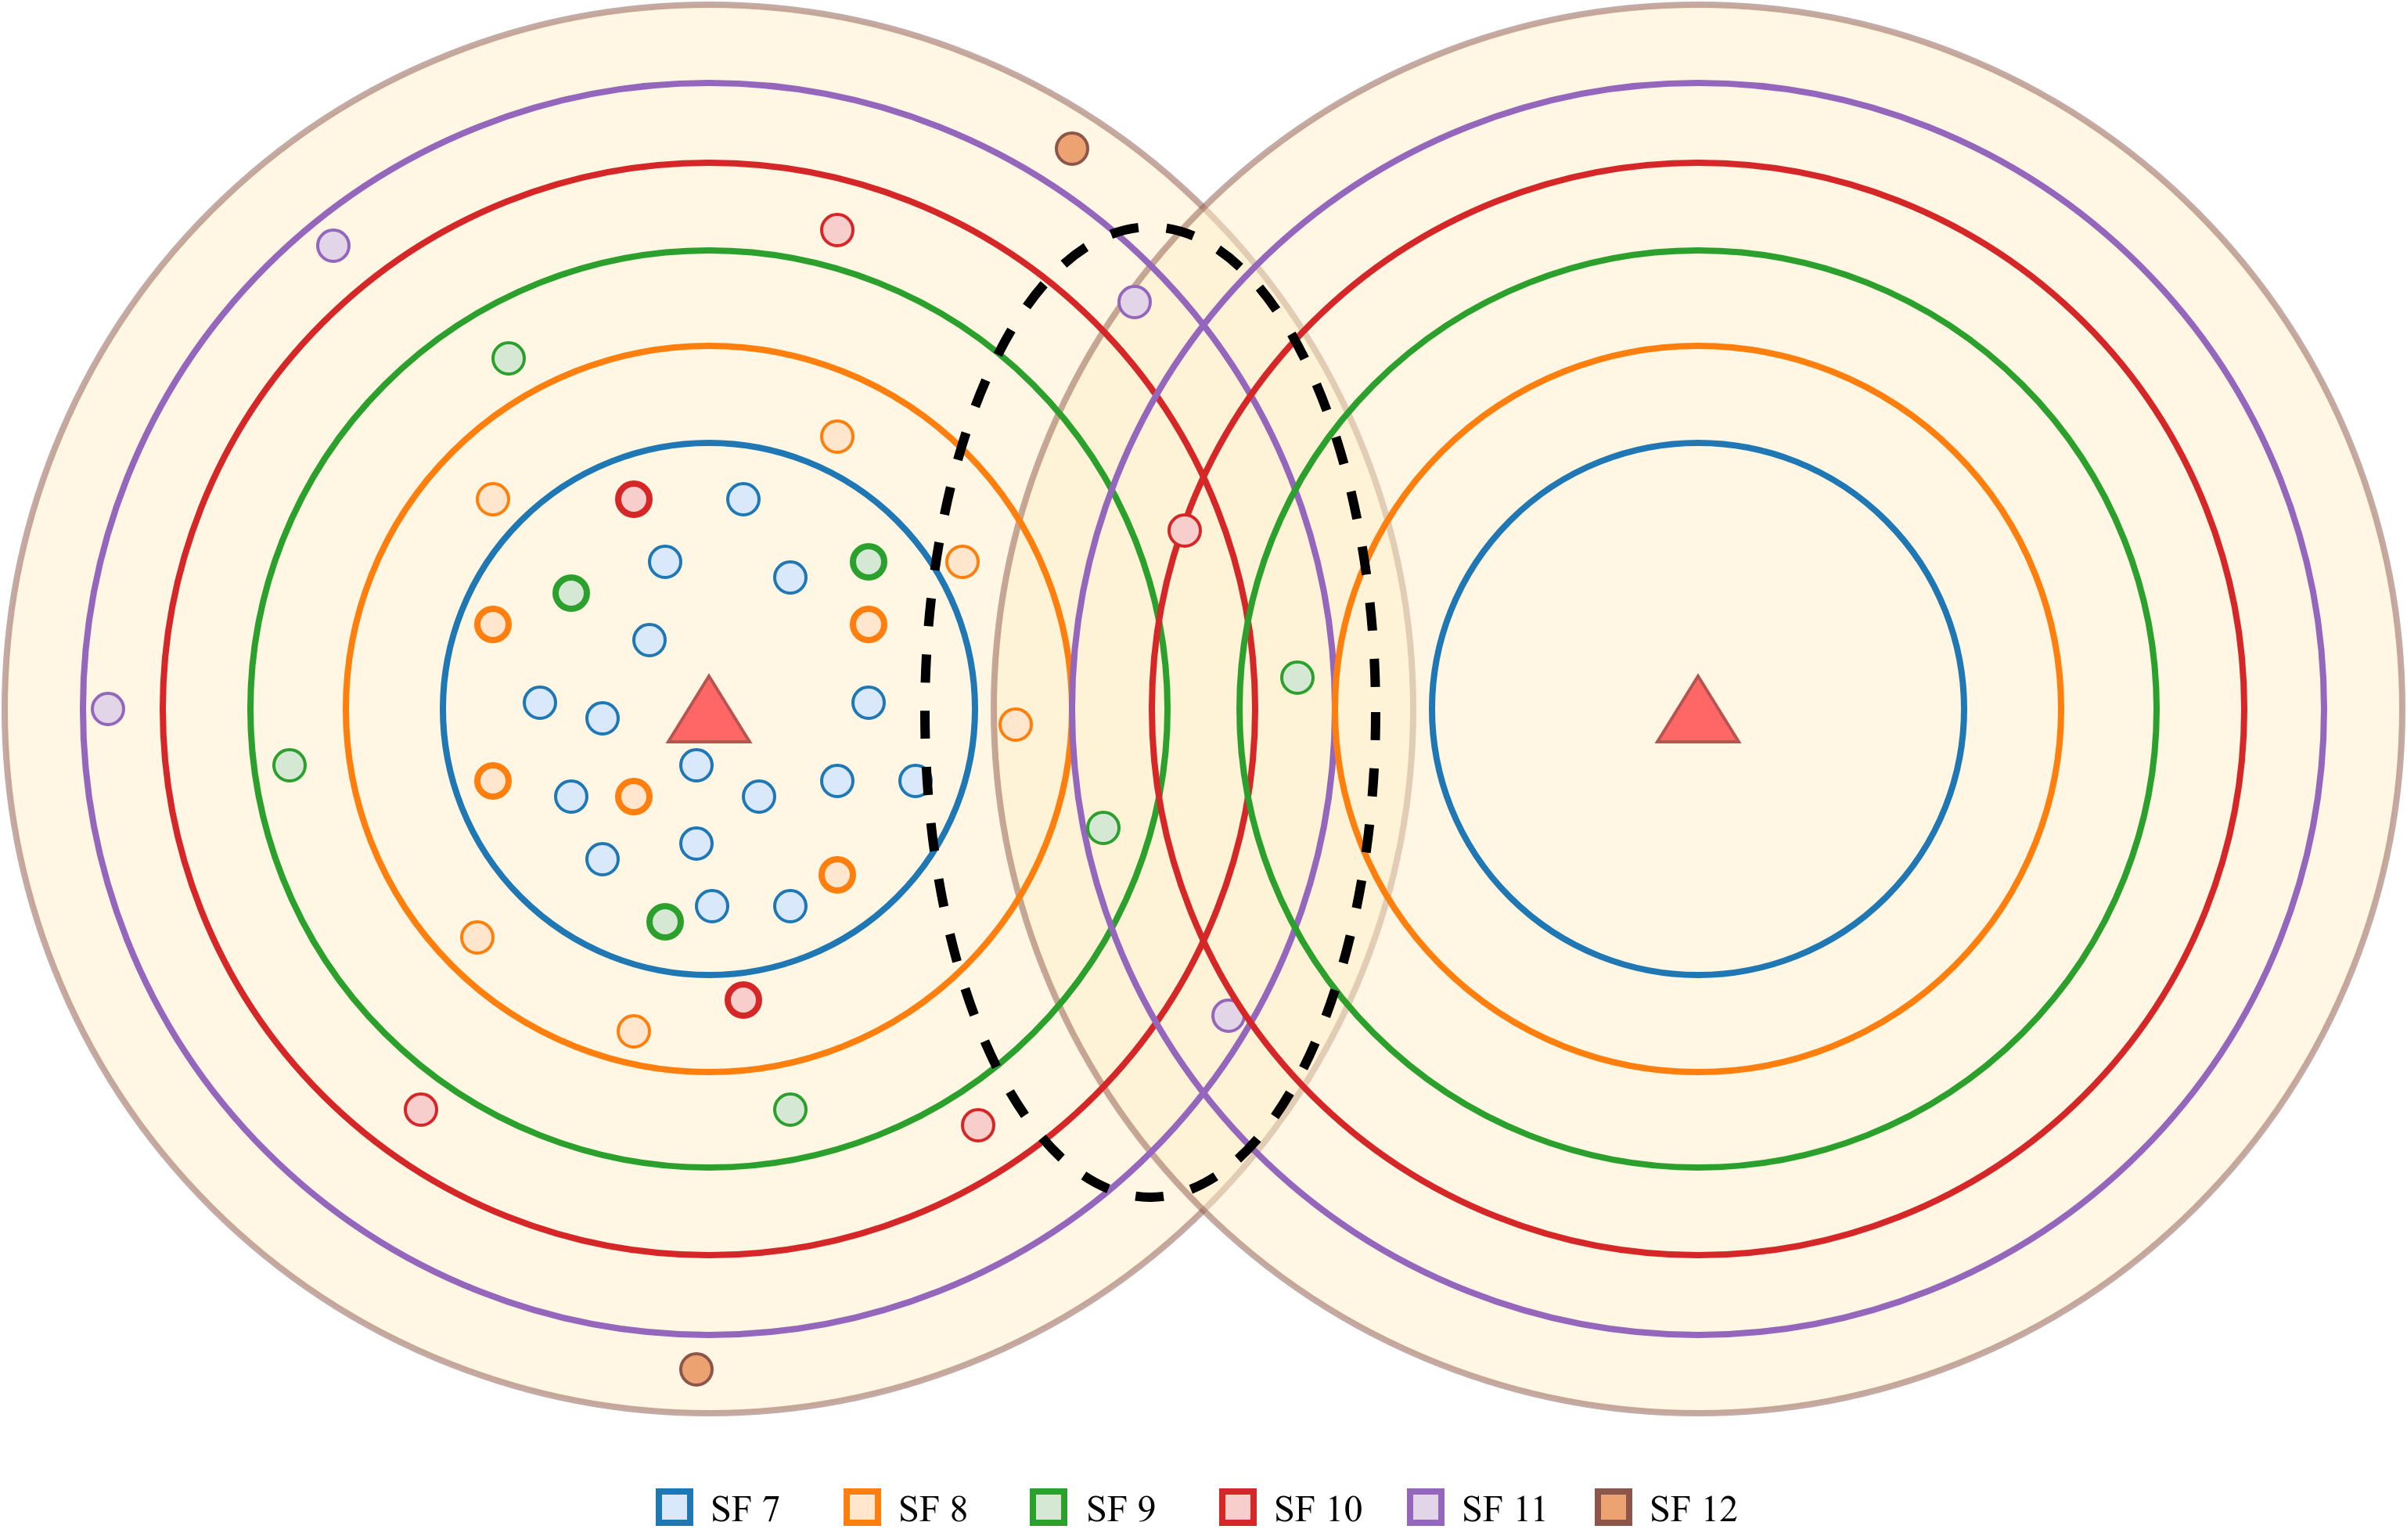
\includegraphics[width=\linewidth]{collision_solution_multi_gw}
\caption{Collision avoidance for intersecting GWs.}
\label{fig:collision_solution_multi_gw}
\end{figure}


\section{Simulation Environment} \label{Simulation Environment}
\par A discrete event simulator is implemented in Python to study the effects of different SF strategies in LoRaWANs. LoRaWAN SF simulation tool source code is available at \cite{simlorasf}. Simulation tool supports custom LoRaWAN topologies as well as randomly generated LoRaWAN topologies. Simulator can generate uniformly distributed circular shape network topology with input parameters; radius (m), number of nodes and number of GWs. Global simulation input parameters are simulation duration (s), packet size (B), packet generation rate (p/s) and SF assignment method. With these inputs, the simulator produces total number of generated packets, number of successfully received packets, number of interfered packets, number of under sensitivity packets, network packet delivery ratio percentage (PDR), network throughput (bps) and total transmit energy consumption (J). Simulator also produces prediction accuracy and confusion matrix for machine learning schemes.

\par The simulator only covers the LoRaWAN Class A devices. Transmissions are always initiated by end nodes in pure ALOHA manner. Nodes generate a new packet randomly according to a Poisson interval for given packet rate parameter. Downlink transmissions are not considered. Downlink transmissions are rare in real world deployments since ISM band regulations dictate duty cycle limit for all devices including GWs.

\subsection{Link Model Employed}
\par Link quality of a wireless system can be expressed by the metric of link budget. Link budget is a measure of all gains and losses from transmitter device to receiver device. Link budget of a wireless link can be calculated as \cite{AN1200.22}:

\begin{equation} \label{eq:expected_rx_power}
P^{dBm}_{RX} = P^{dBm}_{TX} + G^{dB}_{SYS} - L^{dB}_{SYS} - L^{dB}_{PATH}
\end{equation}

\par Where, $P^{dBm}_{RX}$ is the expected receive power at the receiver. $P^{dBm}_{TX}$ is the transmit power of the transmitter. $G^{dB}_{SYS}$ is the system gains such as transmitter and receiver antenna gains. $L^{dB}_{SYS}$ is the system losses such as transmitter and receiver line, circuit, antenna losses. $L^{dB}_{PATH}$ is the propagation path loss between transmitter and receiver antennas in open space. In the simulator, it is assumed that total of system gains $G^{dB}_{SYS}$ and system losses $L^{dB}_{SYS}$ is +7 dB.

\par In the simulator, it is assumed that nodes always select maximum allowed transmit power, which is 14 dBm for European ISM band regulation \cite{lorawan.regional.parameters}. Different channel transmissions are independent from each other. But, in this work we focus on SF orthogonality. Thus, only single channel transmissions are utilized in the simulator.

\par Receive sensitivity of a LoRa GW for different SFs and BWs in dBm unit can be found in \cite{SX1276}. In the simulator, 125 kHz bandwidth receive sensitivities are used.

\par Free space propagation loss is calculated as in \cite{TR136.942}. In this work, it is assumed that $h$ = 15 m and $f$ = 868 MHz.

\par If the received signal power is higher than the GW sensitivity, then signal can be decoded by the receiver successfully when there is no interfering transmission.

\subsection{Interference Model Employed}
\par In the simulator, interference model described in \cite{7996384} is adopted. They use SINR threshold matrix for modeling LoRa interference between simultaneous but different SF LoRa transmissions.

\par It is assumed that there is no other technology interference in the network except LoRa interference. To exploit imperfect orthogonality of different SF transmission, simulator should calculate the effect of different SF transmissions to each other. In simulator, signal to interference plus noise ratio (SINR) threshold matrix from \cite{goursaud:hal-01231221} is used.

\par To decide if a referenced signal is interfered at receiver by an interfering signal, SINR threshold matrix is used. $T_{i,j}$ is SINR margin in dB unit between referenced signal with SF = i and interfering signal with SF = j to correctly decode the referenced signal. If there are more than one interfering signal, referenced signal must satisfy the margin for cumulative sum of all interfering signal received power for each SF \cite{7996384}. Transmission duration of a packet can be calculated by data rate $R_{b}$ and packet size $PS$. Data rate of a LoRa transmission is already expressed in Equation \ref{eq:bit_rate_sf}.

\section{Simulation Results}  \label{Simulation Results}
\par For simulation results in this paper, global simulation parameters are set as follows: packet size = 60 Bytes, simulation duration = 3600 sec, packet generation rate = 0.01 pac/sec.

\par In Figure \ref{fig:sf_pdr}, PDR plot of various SF assignment is shown. Randomly generated network topology radius is set to 3000 meters and number of GWs is set to 1. Increasing SFs increases air time. It increases the number of collisions thus decreases the PDR. High SF schemes gives poor PDR results as the number of nodes increases. Since network topology radius is quite small, all SFs can reach to GW.

\begin{figure}
\centering
\includegraphics[width=\linewidth]{{sf_pdr_r3000_g1_p0.01_s3600}.png}
\caption{PDR for various SFs.}
\label{fig:sf_pdr}
\end{figure}

\par In Figure \ref{fig:gw_pdr}, PDR plot for various number of GWs is shown. Randomly generated topology radius is set to 3000 meters and the lowest SF assignment scheme is used. Increasing number of GWs, decreases the SFs of nodes and decreases air time. This decreases number of collisions, henc, increases the PDR of network when network radius is constant.

\begin{figure}
\centering
\includegraphics[width=\linewidth]{{gw_pdr_r3000_p0.01_s3600}.png}
\caption{PDR for various number of GWs.}
\label{fig:gw_pdr}
\end{figure}

\par In Figure \ref{fig:r_pdr}, PDR plot of various network radius is shown. Number of GW is set to 1 and lowest SF assignment scheme is used. Increasing network radius, increases the number of under sensitivity transmissions thus decreases the PDR of network.

\begin{figure}
\centering
\includegraphics[width=\linewidth]{{r_pdr_g1_p0.01_s3600}.png}
\caption{PDR for various network radii.}
\label{fig:r_pdr}
\end{figure}

\par PDR plot of the lowest SF scheme and the smart prediction schemes are shown in Figure \ref{fig:prediction_pdr}. Randomly generated network radius is set to 5000 meters and number of GWs is set to 3. Prediction model needs nodes' locations and three GWs are enough to locate nodes positions by triangulation. In Table \ref{table:prediction_pdr}, PDR values for various network radii are presented. Both smart SVM and smart DTC schemes give better PDR than lowest SF schemes when number of nodes increases. Increasing number of nodes, increases number of interferences. Smart schemes improve network performance when LoRa interference is high. Moreover, smart schemes give better results when nodes are deployed closer to the GW, since nodes have margin to increase their SFs when they are deployed closer to the GW. If a node is far away from GW, then smart schemes cannot increase the SF to avoid interference since the assigned SF is already high.

\par In Table \ref{table:prediction_accuracy}, prediction accuracy of smart SVM and smart DTC schemes are presented for various network radii and number of nodes. Prediction accuracy is not directly proportional to network PDR. Correct prediction of an interfered transmission may not increase the PDR but increases the accuracy. Mart DTC gives better PDR results than smart SVM, even overall SVM prediction accuracy is high.


\begin{figure}
\centering
\includegraphics[width=\linewidth]{{prediction_pdr_r5000_g3_p0.01_s3600}.png}
\caption{PDR for lowest SF and smart SF schemes.}
\label{fig:prediction_pdr}
\end{figure}

\begin{table}
\centering
\caption{PDR for lowest SF and smart SF schemes.}
\label{table:prediction_pdr}
\begin{tabular}{|c|c|c|c|c|c|}
\hline
\multicolumn{3}{|c|}{\multirow{2}{*}{}}                            & \multicolumn{3}{c|}{\textbf{Number of Nodes}} \\ \cline{4-6}
\multicolumn{3}{|c|}{}                                             & 100           & 500           & 1000          \\ \hline
\multirow{12}{*}{\textbf{R (m)}} & \multirow{3}{*}{3000}  & Lowest & 97.8          & 86.0          & 72.3          \\ \cline{3-6}
                                 &                        & SVM    & 98.0          & 88.2          & 75.2          \\ \cline{3-6}
                                 &                        & DTC    & 97.8          & 89.8          & 78.7          \\ \cline{2-6}

                                 & \multirow{3}{*}{5000}  & Lowest & 96.8          & 85.5          & 71.2          \\ \cline{3-6}
                                 &                        & SVM    & 98.0          & 87.8          & 74.8          \\ \cline{3-6}
                                 &                        & DTC    & 97.7          & 90.2          & 79.8          \\ \cline{2-6}

                                 & \multirow{3}{*}{7000}  & Lowest & 97.2          & 87.5          & 76.8          \\ \cline{3-6}
                                 &                        & SVM    & 98.2          & 88.8          & 78.6          \\ \cline{3-6}
                                 &                        & DTC    & 97.8          & 90.7          & 81.6          \\ \cline{2-6}

                                 & \multirow{3}{*}{10000} & Lowest & 98.2          & 90.3          & 81.5          \\ \cline{3-6}
                                 &                        & SVM    & 98.3          & 90.3          & 81.9          \\ \cline{3-6}
                                 &                        & DTC    & 98.3          & 90.6          & 81.9          \\ \hline
\end{tabular}
\end{table}

\begin{table}
\centering
\caption{Prediction accuracy of SVM and DTC classifiers.}
\label{table:prediction_accuracy}
\begin{tabular}{|c|c|c|c|c|c|}
\hline
\multicolumn{3}{|c|}{\multirow{2}{*}{}}                        & \multicolumn{3}{c|}{\textbf{Number of Nodes}} \\ \cline{4-6}
\multicolumn{3}{|c|}{}                                         & 100           & 500           & 1000          \\ \hline
\multirow{8}{*}{\textbf{R (m)}} & \multirow{2}{*}{3000}  & SVM & 82.4          & 70.4          & 71.7          \\ \cline{3-6}
                                &                        & DTC & 86.0          & 67.3          & 70.4          \\ \cline{2-6}

                                & \multirow{2}{*}{5000}  & SVM & 79.5          & 69.0          & 71.1          \\ \cline{3-6}
                                &                        & DTC & 84.5          & 67.3          & 69.5          \\ \cline{2-6}

                                & \multirow{2}{*}{7000}  & SVM & 79.5          & 70.6          & 71.2          \\ \cline{3-6}
                                &                        & DTC & 84.5          & 67.7          & 69.2          \\ \cline{2-6}

                                & \multirow{2}{*}{10000} & SVM & 79.2          & 74.4          & 76.1          \\ \cline{3-6}
                                &                        & DTC & 83.8          & 70.7          & 74.3          \\ \hline
\end{tabular}
\end{table}

\par For space constraints, we omit results like network throughput and total transmit energy consumption. We invite readers to experiment the simulation tool with the parameters they like. \cite{simlorasf}.


\section{Conclusion} \label{Conclusion}
\par In this paper, we present a discrete event simulator which is developed from scratch to study network performance of LoRaWAN and evaluate different SF assignment schemes. Moreover, we show how SF collisions can be avoided, hence, we propose a machine learning based solutions called smart DTC scheme and smart SVM scheme. We present simulation results for the lowest SF assignment scheme and the proposed schemes. Simulation results show that, the proposed smart schemes can increase network performance for LoRaWAN networks, especially, when the nodes are deployed close to GWs.

\par As for future work, transmit power optimization can be included to the proposed smart schemes. In this paper, it is assumed that nodes always use maximum transmit power for uplink transmission, however nodes close to GWs can decrease transmit power to save energy. This will make transmissions more vulnerable to interference thus requires extra care. Moreover, other machine learning methods can be investigated for SF assignment enhancement. Reinforcement learning could be a good candidate. Also, other transmission parameters such as node id and transmission time can be included to the proposed scheme to the improve performance.


\section*{Acknowledgment}
\par This work is supported by Turkish Ministry of Development and Istanbul Technical University researcher support program under the Grant No. ITU-AYP-2017-1.


\bibliographystyle{IEEEtran}
\bibliography{references}

\end{document}
